\section{Cookie-Storage}
\label{clientcookie}

Damit sich ein User des Clients nicht nach jedem App-Neustart erneut mit seinen Logindaten anmelden muss,
werden dessen E-Mail-Adresse sowie der generierte Session-Token, der nach einem erfolgreichem Login erhalten wird, 
in Form von Cookies im externen Speichers des Geräts abgespeichert.

% https://flutter.dev/docs/cookbook/persistence/key-value

Damit dies plattformunabhängig funktioniert, wird das \lstinline{shared-preferences}-Package von Flutter
verwendet.
Dieses Plugin wrapped die \lstinline{NSUserDefaults} von iOS und die \lstinline{SharedPreferences} von Android,
wodurch Key-Value-Paare persistent unabhängig vom Betriebssystem abgespeichert werden können.

Damit die Daten, die im Cookie-Storage gespeichert sind, global in der App verfügbar sind, wird in jener Klasse das \textit{Singleton-Design-Pattern} angewendet. Dieses ermöglicht, dass immer dieselbe, einzige Instanz dieser Klasse aufgerufen wird, anstatt immer neue Objekte per Konstruktor anzulegen.

Dart hat hierfür eine eigene syntaktische Lösung:

\begin{code}[H]
    \centering
    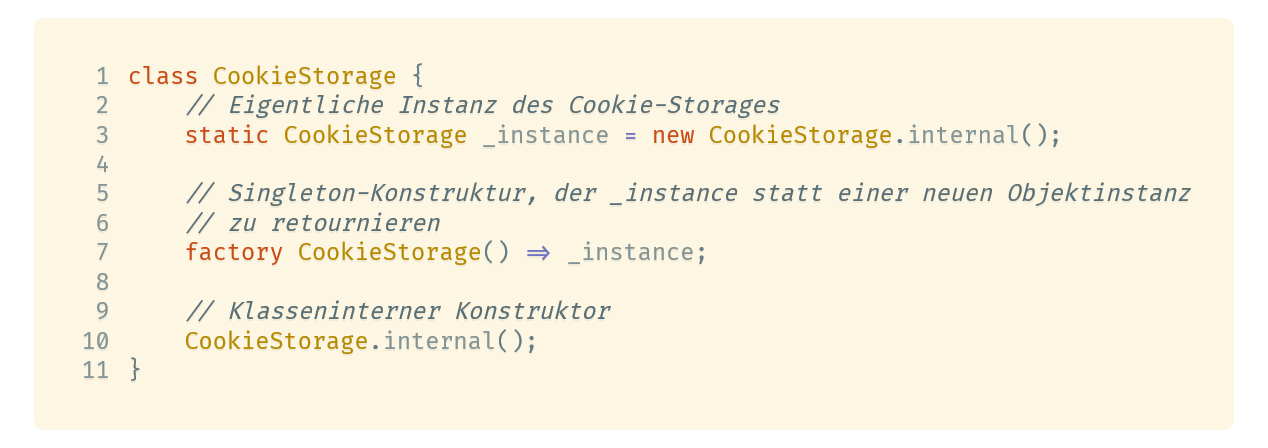
\includegraphics[width=1\textwidth]{images/Client/util/cookie-storage/cookieStorageSingleton.png}
    \vspace{-25pt}
    \caption{Dart's syntaktische Lösung für die Erstellung eines Singletons}
\end{code}

Innerhalb der Klasse besitzt der Cookie-Storage zusätzlich eine Map \lstinline{Map<String, String>},in der die Key-Value-Paare nochmals abgespeichert werden, damit sie in dafür notwendigen Situationen synchron abgefragt werden können.

Das Speichern und Abfragen von Werten, die im externen Speicher des Geräts gespeichert sind erfolgt, über eine Instanz der \textit{SharedPreferences}:

\begin{code}[H]
    \centering
    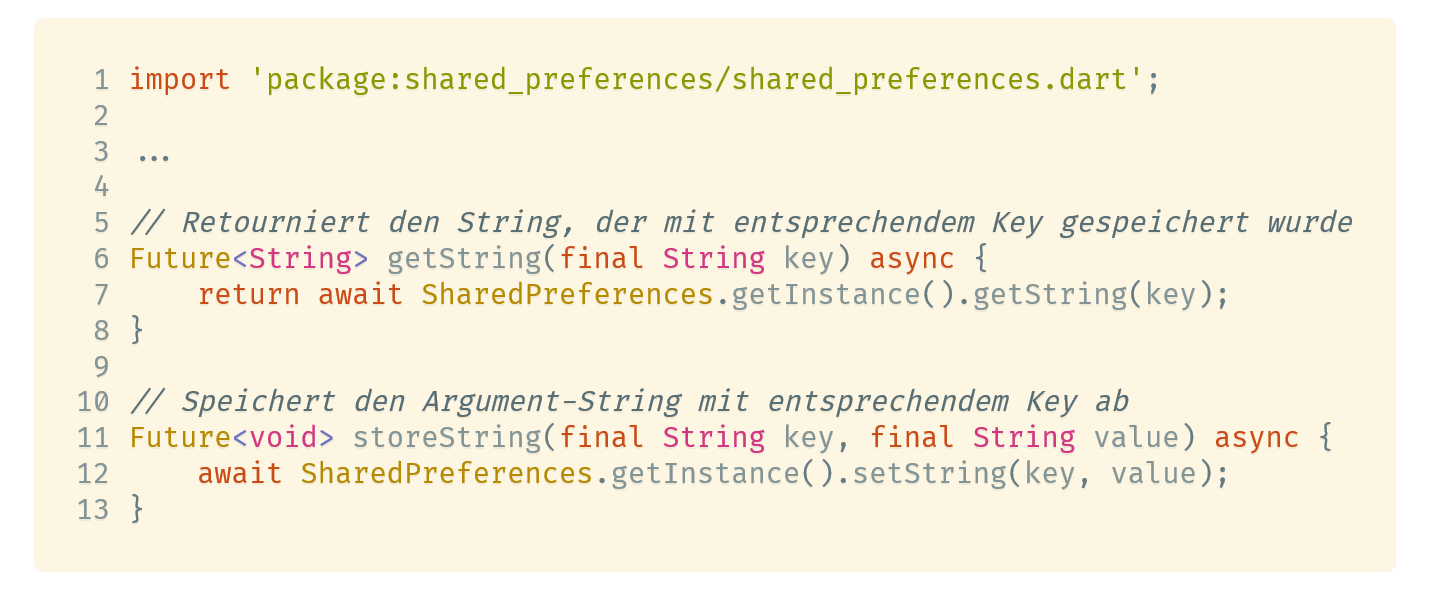
\includegraphics[width=1\textwidth]{images/Client/util/cookie-storage/sharedPreferences.png}
    \vspace{-25pt}
    \caption{Speichern von Key-Value-Pairs in den externen Gerätespeichern}
\end{code}

Damit die gespeicherten Daten auch in der App persistent abgerufen werden können, gibt es klassenintern
im Cookie-Storage vorgefertigte, statische Keys sowohl für den Session-Token als auch für die User-E-Mail-Adresse:

\begin{code}
    \centering
    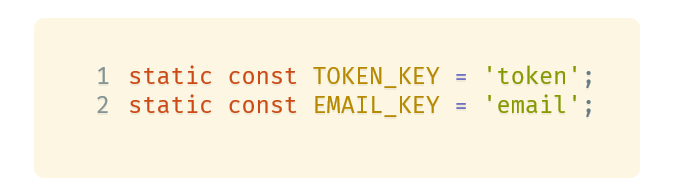
\includegraphics[width=1\textwidth]{images/Client/util/cookie-storage/cookieKeys.png}
    \vspace{-25pt}
    \caption{Definieren von statischen Key-Strings für erhöhte Typsicherheit}
\end{code}

So können Fehler, die durch Tippfehler oder falsche Angaben des Keys beim Abspeichern bzw. Abfragen
von Werten entstehen, zur Gänze verhindert werden.

Anstatt den Key also manuell anzugeben, kann dieser nun simpel über die statische Klassenvariable
aufgerufen werden.

\begin{code}
    \centering
    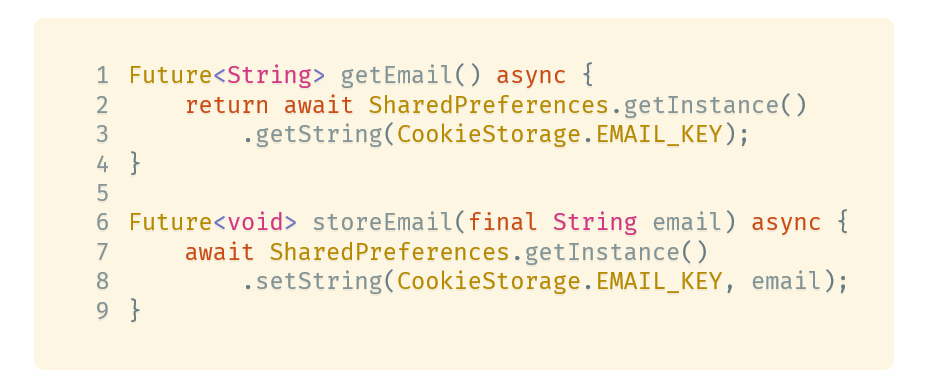
\includegraphics[width=1\textwidth]{images/Client/util/cookie-storage/getAndStoreWithStaticKey.png}
    \vspace{-25pt}
    \caption{Verwalten von Cookie-Daten mithilfe oben definierter Static-Keys}
\end{code}